\documentclass{report}


\input{~/Documents/Licence/LaTeX_Models/Header_Cours.tex}

\usepackage{fancyhdr}


\setlength{\headheight}{50pt}


\lstset{%
  language=Java,
  basicstyle   = \footnotesize,
  keywordstyle =    \color{magenta},
  keywordstyle = [2]\color{orange},
  commentstyle =    \color{gray}\itshape,
  stringstyle  =    \color{cyan},
  numbers      = left,
  frame        = single,
  framesep     = 2pt,
  aboveskip    = 1ex
}



\begin{document}

% ==================================== Titre =========================================================



\title{Morpy}
\author{Axel Pigeon \& Anaïs Pertoldi-Blanc}

\pagestyle{fancy}
\lhead{Rapport de Projet Réseau}
\chead{}
\rhead{\includegraphics[width=0.07\textwidth]{Logo.png}}
\lfoot{}
\cfoot{\thepage}
\rfoot{}
\renewcommand\headrulewidth{1pt}
\renewcommand\footrulewidth{0pt}


\makeatletter
  \begin{titlepage}
  \centering
      {\large \textsc{Institut National Universitaire Champollion}}\\
      \textsc{Rapport Réseau}\\
    \vspace{1cm}
    \begin{center}
        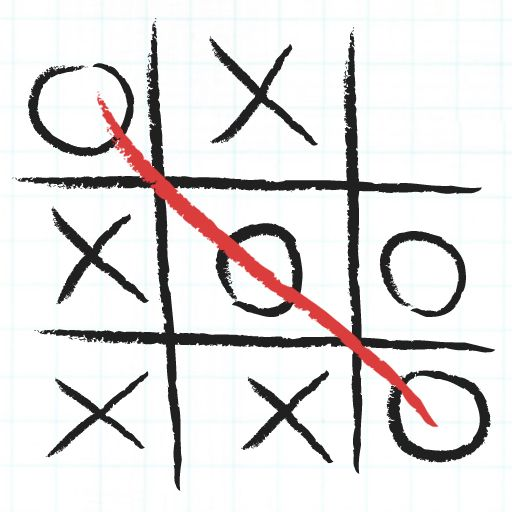
\includegraphics[width=0.50\textwidth]{couverture.jpg}
    \end{center}
    \vspace{1cm}
       {\Huge \textbf{\@title}} \\
    \vspace{2em}
        {\large \@author} \\
  \end{titlepage}
\makeatother


% \tableofcontents

\newpage


% ==================================== Corps =========================================================

\raggedright
\justifying

% ==================================== Introduction à la Cryptographie  =========================================================


\section*{Introduction}

Durant notre L2 de Licence Informatique à l'INU Champollion, un projet de Morpion en réseau programmé en Java nous a été proposé. Ce rapport présente en profondeur le fonctionnement de \emph{Morpy}.

Tout d'abord nous présenterons les différentes classes utilisées ainsi que leur fonctionnement dans les grandes lignes.
Ensuite, nous détaillerons la méthode de connexion entre les deux joueurs ainsi que le déroulement d'une partie.
Enfin, nous finirons par un petit manuel d'utilisation, même si l'utilisation est très simple.


\section*{Structure Générale de \emph{Morpy}}

\emph{Morpy} est composé de plusieurs classes gravitant toutes autour de \textbf{\texttt{MorpionCMD}}. 

\subsection*{Une jeu construit autour de sa version CMD}

Cette classe contient tout les algortihmes et méthodes essentiels au fonctionnement de l'application.
Les méthodes que l'on pourrait qualifier de plus importantes (outre le constructeur) de la classe \texttt{MorpionCMD} sont les suivantes :
\begin{itemize}
    \item \textbf{\texttt{startGame()}} : elle permet de réellement lancer le jeu en faisant choisir aux joueurs leur \texttt{connexionMode} (serveur ou client), indispensable au déroulement de la partie.
            Elle établit la connexion entre les deux joueurs via les classes \textbf{\texttt{Client}} et \textbf{\texttt{Serveur}} et ensuite de lance la partie.
    \item \textbf{\texttt{tour()}} : Cette méthode est appelée autant de fois que nécessaire tant que la partie n'est pas terminée. Elle se déroule selon 4 étapes :
            \begin{enumerate}
                \item Récupération de la grille de jeu dans le Socket
                \item Vérification que le joueur adverse n'a pas joué un coup gagnant ou que la partie est terminée 
                \item Entrée du nouveau coup 
                \item Vérification que le coup joué n'est pas gagnant ou que la partie n'est pas finie 
                \item Envoi de la grille avec le nouveau coup joué
            \end{enumerate}
    \item \textbf{\texttt{affiche()}} qui écrit tout simplement la grille 
    \item \textbf{\texttt{partieFinie()}} qui renvoie \texttt{true} si la partie est finie (un joueur a gagné ou la grille est pleine) ou \texttt{false} sinon.
    \item \textbf{\texttt{envoyer()}} qui permet d'envoyer la grille de jeu à l'adversaire via le socket. Les méthodes \texttt{envoyer()} et \texttt{recevoir()} sont exactement les mêmes pour les deux joueurs. Leur comportement est entièrement défini selon l'attribut \textbf{\texttt{connexionMode}} qui vaut \texttt{true} si l'utilisateur est connecté en serveur ou \texttt{false} si il est connecté en tant que client.
    \item \texttt{recevoir()} qui lit la chaîne de caractère envoyée dans le socket, la traite pour récupérer les valeurs de chaque case et met à jour d'attribut \texttt{grille}.
\end{itemize}




\subsection*{Error 404 !!!}

Ensuite, vient le tour des classes \texttt{Serveur} et \texttt{Client}. Leur utilisation n'est pas spécialement nécessaire, nous aurions pu ajouter ce qu'elles font dans la classe \texttt{MorpionCMD} mais nous avons fait le choix de strictement compartimenter la partie "morpion" et la partie "réseau".
La première étape de développement a donc été celle de ces deux classes, sans elles, rien de fonctionne. 
Grâce au compartimentage, une fois qu'elles ont étés opérationnelles, la partie réseau ne nous posait plus de problèmes, il suffisait "seulement" de rajouter la couche application dessus. 
Pour la connexion entre les deux joueurs, nous utilisons des Socket. Un socket est un processus de communication bidirectionnelle entre deux hôtes. Concrètement, une fois la connexion établie entre les deux joueurs, le socket fonctionne comme un "tunnel" par lequel les utilisateurs peuvent envoyer des données des deux côtés.

Ici, dans les classes \texttt{Serveur} et \texttt{Client}, les méthodes \texttt{send...()} et \texttt{read....()} permettent d'écrire ou de lire du contenu dans le socket. Ces méthodes sont ensuite utilisées par \texttt{envoyer()} et \texttt{recevoir()} pour l'échange des grilles de jeu au cours de la partie.


\subsection*{Port de lunettes conseillé pour l'utilisation de la version graphique...}


Enfin, la classe \texttt{MorpionGraph} est la version graphique de \emph{Morpy}. Elle hérite de \texttt{MorpionCMD}, ce qui nous a permis de récupérer toutes les méthodes nécessaire au fonctionnement de l'application sans avoir à les toutes réécrire, notamment grâce à notre décision de tout compartimenter.
Elle fonctionne sensiblement de la même façon que \texttt{MorpionCMD} sauf que toutes les interactions avec la ligne de commande ont étés remplacées par une interface graphique. Celle-ci a été réalisée avec \emph{Swing}, une bibliothèque d'interface graphique de \emph{Java} développée par \emph{Oracle}.


\section*{Déroulement d'une partie}

Le déroulement d'une partie est assez simple et est exactement le même pour la version CMD que pour la version graphique. Tout commence par l'exécution de \texttt{Main.java} qui demande à l'utilisateur à quelle version de \emph{Morpy} il souhaite jouer.
En fonction de cela, la version demandée est lancée et le jeu peut commencer... 

Dans les deux cas, la méthode \texttt{startGame()} est lancée pour essayer d'établir une connexion entre les deux joueurs. Si le joueur choisit d'être le serveur, il doit communiquer son adresse ip (qui s'affiche sur l'écran) à son adversaire. Celui-ci doit alors l'entrer pour établir la connexion.
Si cela ne fonctionne pas, une erreur apparaît et l'application se ferme. Sinon, la partie peut commencer.

On entre ensuite dans une boucle qui lance la méthode \texttt{tour()} tant que la condition \texttt{partieFinie} ne vaut pas \texttt{true}.

Lors de la première exécution de \texttt{tour()} le serveur commence à jouer et le client attend la réception du coup. L'utilisation des socket permet "d'attendre" l'écriture de la grille dans le socket avant la saisie du coup par le joueur et ainsi un jeu "coup par coup".
Nous avons délibérément fait le choix d'envoyer toute la grille de jeu à chaque coup dans le socket. La gestion de la validité du coup entré se fait donc par le joueur qui entre le coup en local. D'un point de vue sécurité, ce n'est pas optimal car un joueur pourrait modifier le code pour envoyer une grille gagnante dès le premier coup.
La méthode est discutable mais cela nous permet de nous affranchir de la synchronisation des grilles de jeu des deux joueurs et ainsi limiter le nombre d'échanges dans le socket.


\section*{Bonus : Améliorations Possibles}

La liste des choses à améliorer est très longue mais certains de ces items sont peut être plus importants. 

Tout d'abord, \emph{Morpy} est très limité, en effet, il n'existe pas de version permettant à deux utilisateurs de jouer sur la même machine, il faut nécessairement deux machines.

Ensuite, la gestion des erreurs dûes à la connexion est archaïque. Dès qu'une erreur survient un simple message apparaît et l'application se ferme. Une description de l'erreur et des options pour fixer le problème seraient de bonnes idées. 
Concernant la gestion des erreurs toujours, il n'est pas conseillé de se tromper lors de la saisie d'un choix ou de l'adresse ip... \emph{Morpy} supporte difficilement les fautes de frappes.

Enfin, l'amélioration de l'esthétique de la version graphique serait visuellement appréciable. Celle-ci a été developpée en seulement quelques jours donc l'accent a été mis sur le fait qu'elle soit fonctionnelle et non pas esthétique.


\section*{Manuel d'utilisation}

\begin{lstlisting}
    public class Manuel {

        public static void main(String[] args) {
            System.out.println("Suivez les instructions affichees a lecran");
        }
    }
    // End
\end{lstlisting}



\section*{Conclusion}

Pour conclure, le développement de \emph{Morpy} nous a permis de découvrir de nouvelles fonctionnalités parmi l'infinité que propose \emph{Java}, notamment les Socket.
De plus, ce projet nous a demandé de mobiliser à la fois nos connaissances en Réseau et nos aptitudes de programmation Java, choses que nous faisions séparément jusqu'à maintenant. 
Plus globalement, cette seconde année de Licence nous permet de nous rendre compte de la puissance des outils que nous utilisons, notamment au travers des projets que nous avons à réaliser.
Projets qui constituent le summum de plusieurs semestre d'introduction.









%\begin{figure}[!ht]
%    \center 
%    \includegraphics[scale=0.05]{image_enigma.jpeg} %l'image est réduite de moitié   
%    \caption{Photo d'une machine Enigma de l'armée Allemande à trois rotors.}
%\end{figure}





\end{document}